\chapter{Results}

% source code structure
\section{Source Code Structure}
\begin{figure}[h!]
	\Large
	\centering
	\caption{Source code structure of this project.}
	\label{fig:source-code-structure}
	\begin{minipage}{6cm}\dirtree{%
			.1 monkeyOffice.
			.2 config.
			.2 lib.
			.2 middleware.
			.2 model.
			.3 document.
			.2 public.
			.3 font-awesome.
			.3 fonts.
			.3 images.
			.3 javascripts.
			.3 stylesheets.
			.4 dist.
			.5 css.
			.5 js.
			.4 login.
			.2 routes.
			.3 api.
			.3 download.
		}
	\end{minipage}
		\begin{minipage}{6cm}\dirtree{%
				.1 monkeyOffice.
				.2 test.
				.3 integration.
				.4 routing.
				.5 api.
				.3 unittest.
				.4 model.
				.5 document.
				.2 uploads.
				.2 utility.
				.2 views.
				.3 dms.
				.3 errors.
				.3 layouts.
			}
		\end{minipage}
\end{figure}

\newpage 

From \ref{fig:screenshot_login}, at first time user have click the sign up link to create a new account for accessing into the main system which is another page \ref{fig:screenshot_signup}

\begin{figure}[H!]
	\centering
	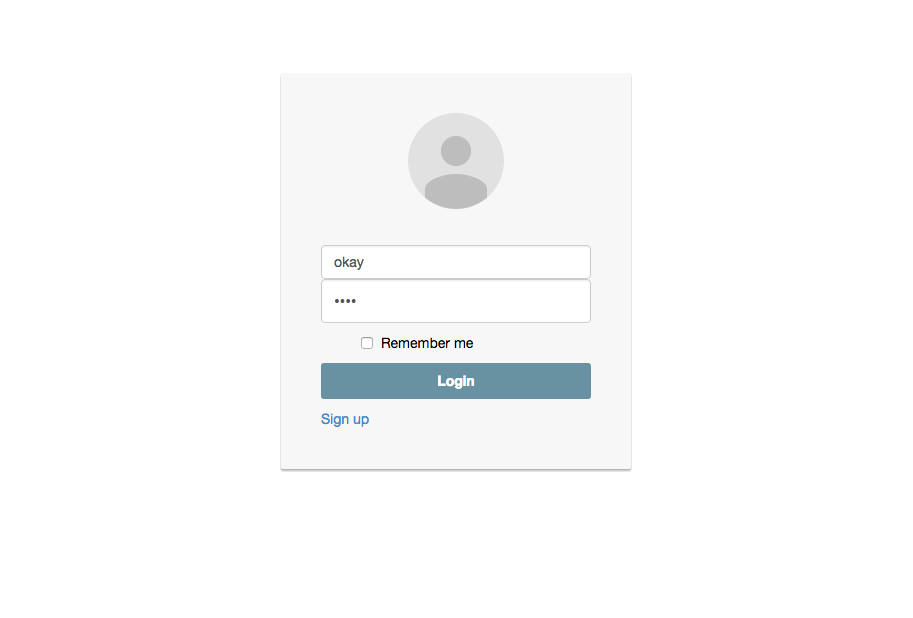
\includegraphics[scale=0.4]{res/Screen_Shot1}
	\caption{Log in page on website}
	\label{fig:screenshot_login}
\end{figure}

\begin{figure}[H!]
	\centering
	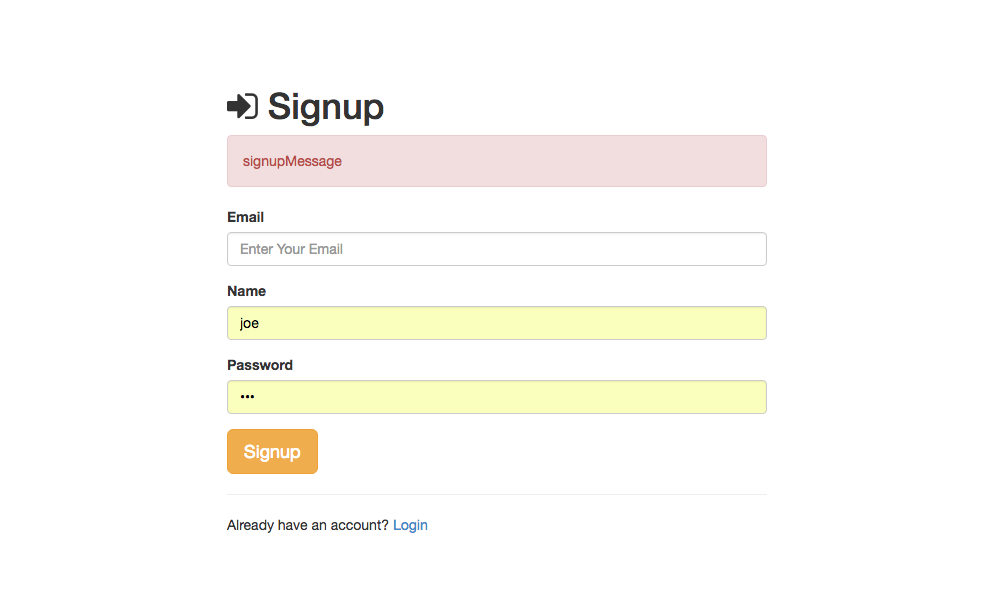
\includegraphics[scale=0.4]{res/Screen_Shot3}
	\caption{Sign up page on website}
	\label{fig:screenshot_signup}
\end{figure}


\begin{figure}[H!]
	\centering
	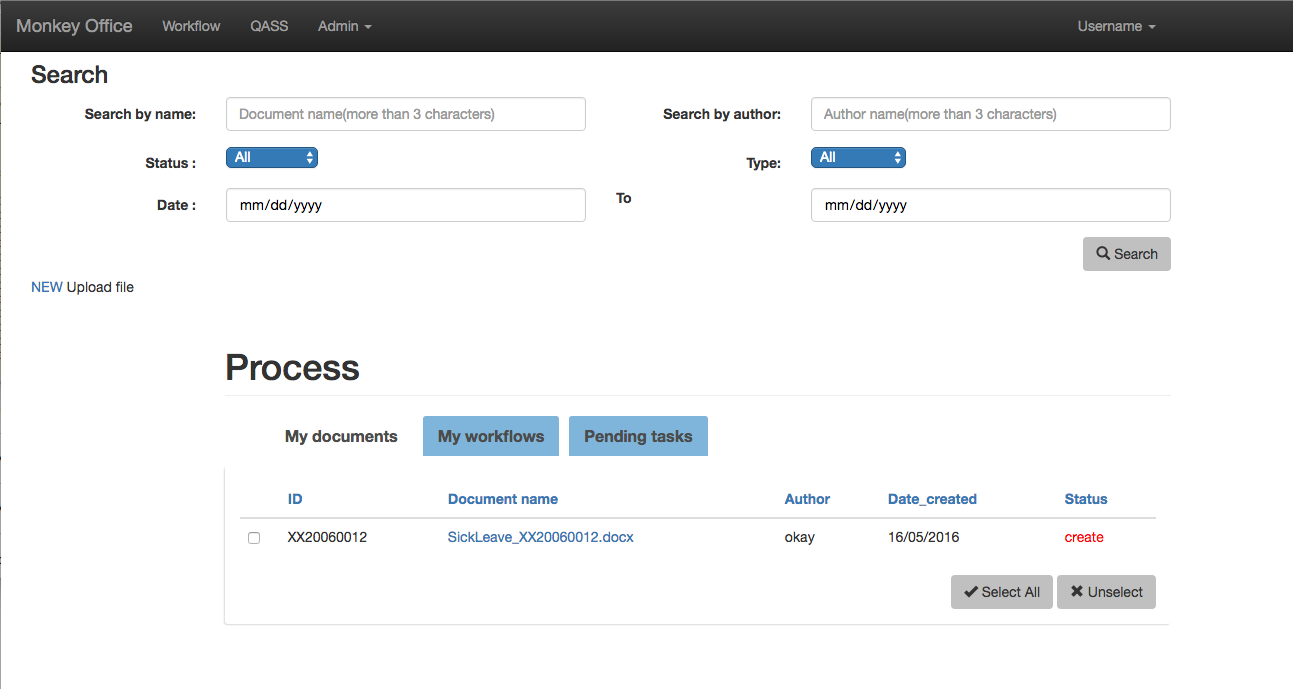
\includegraphics[scale=0.3]{res/Screen_Shot2}
	\caption{Home page on website}
	\label{fig:screenshot_home}
\end{figure}

After that when the user logged in 	user can see the list of documents, workflows and pending tasks so user can click the name of document to get in to view more information of this that user selected, also user can searching the documents by name of document, author name,created date,type of document, and status. \ref{fig:screenshot_home}

% tour the interface

% demonstration

% testing

